% !TeX root = ../main.tex
% Add the above to each chapter to make compiling the PDF easier in some editors.

\chapter{Simulation Setup}\label{chapter:simulation_setup}
The Experiment Setup can be divided into two phases, one is set up the simulation and collect data from the simulated setup. We call title this two-section as Simulation and Data Collection respectively.
In this section we describe the detailed information for the simulation software and how we gathered data from the simulation and preprocessed the data to feed in the CNN algorithm.

We use simulated data because its easier to deal without any noise and doesn't need calibration and registration. The other advantages of the simulated data are that the simulated environment is ideal for this kind of experiment without any noisy data and its ideal for the analysis of the result before using it into the real world scenario and compare with it.

We obtained the from the simulation as .txt formate. then we processed the data and convert the data points in csv formate to use in our CNN model.

\section{Simulation}
As for the simulation we need to choose a simulation software that fulfills our requirement for simulating IMUs and moving the sensors on a flat plane on a predefined path. The other crucial requirements were, the data must be faultless and noise-free. For example, the item that had been utilized to mount the IMUs needed to move openly satisfying Six Degrees of Freedom (6DoF). 

Moreover, the estimations from the virtual IMUs must be as exact as conceivable to imitate a real situation. We had fewer options for the simulation software to choose from. Among the simulation software we checked for our simulation MATLAB and CoppeliaSim Robotics were better performing.

\subsection{Simulation software}
After intensive investigation, we chose to go with the CoppeliaSim Robotics Education version for our simulation tool. Beforehand this product was known as V-Rep by Coppelia Robotics. One of the primary purposes behind picking this simulation tool is the assortment of accessible simple to utilize alternatives to mimic genuine situations. This product is created to recreate genuine situations for various mechanical parts for example Robot arms, Hexapods. It additionally has a wide scope of different segments for reproduction purposes. For instance – Infrastructure, furniture, family unit things, office things, and even people for reenactment purposes. This product offers a scope of usable virtual sensors for example – accelerometers, spinners, vision sensors, laser scanner, GPS sensors, and so forth. 

The training adaptation is free for all. Since we didn't need to stress over the frequencies of various IMUs since every one of them is reproduced, the CPU recurrence made a difference the most while gathering the information. To analyze the reason, we ran the recreation on various CPU load. For example, with 4 IMUs and no other application running on the foundation, it took roughly 73 minutes to gather 1,06,437 information focuses. In a similar arrangement, however, with Google Chrome running on the foundation, the reenactment could just gather 47,509 information focuses on a similar time. It is required to run the reproduction remain solitary to get around the comparative number of information that focuses on a comparable time period.

In the following section we will describe the the components of the CoppeliaSim Robotics and how we used it to create the simulation 

\subsection{Scene Object}


\begin{figure}[h!]
  \centering
  \begin{subfigure}[b]{0.4\linewidth}
    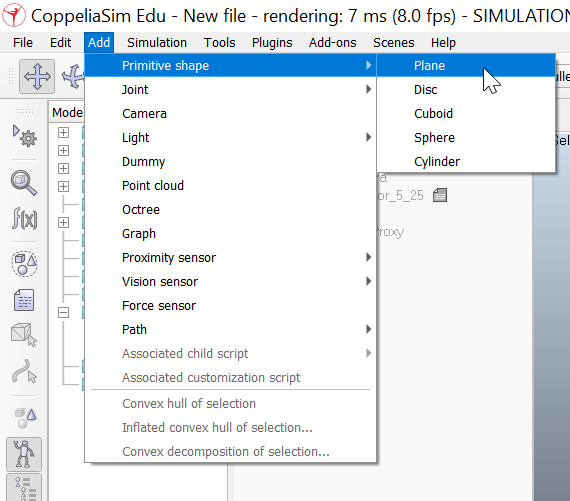
\includegraphics[width=\linewidth]{figures/adding_2d_plane.png}
    \caption{2D plane to the scene.}
  \end{subfigure}
  \begin{subfigure}[b]{0.4\linewidth}
    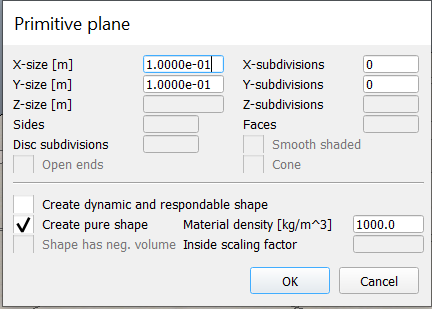
\includegraphics[width=\linewidth]{figures/config_plane.png}
    \caption{Plane Configaration.}
  \end{subfigure}
 \begin{subfigure}[b]{0.6\linewidth}
    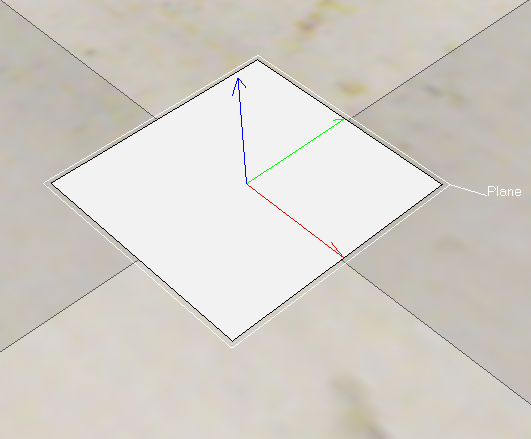
\includegraphics[width=\linewidth]{figures/plane.png}
    \caption{Created 2D plane.}
  \end{subfigure}
  \caption{Creating scene object.}
  \label{fig:scene_object}
\end{figure}

To recreate a real-world like situation, the main thing we required was an object for the scene. The object would represent the qualities of a moving segment in the simulated scenario

For our investigation, we required an object to contain the IMUs that would move along on a pre-characterized way. Obviously, 6 DoF must be guaranteed to make however much as could reasonably be expected accurate data. For our first methodology, we utilized effectively accessible predefined shapes that built-in the software. The software gives a number of predefined shapes such as plane, circle, cuboid, circle, and cylinder. We picked to utilize a two-dimensional plane as our object since it is the nearest to our model scenario. 



The plane is sufficiently large to contain at least 16 IMUs which is the most noteworthy number of IMUs we chose to utilize. The examples for putting the IMUs on the plane had been chosen together which would in the end help us to get the most ideal and solid information. 

To add our ideal object to the scene, the following steps were :
\begin{enumerate}
  \item Click on ‘Add’ on the menu bar.
  \item Go to the first option; ‘Primitive Shape’.
  \item Click on ‘Plane’ to add a two dimensional plane in our scene.
  \item No change needed in the ‘Primitive plane’ dialog box and click ‘OK’.
\end{enumerate}


\subsection{Inertial Measurement Units}

The next task is to add IMUs (Inertial Measurement Units) into our plane. The IMU containes an accelerometer and a gyroscope sensor. In the sensor section of the simulation tool, there is no IMU sensor out of the box but there are an accelerometer and a gyroscope sensor. To create IMU we combined these 2 sensors and added to to our plane. 

To add one of those sensors to our scene, the following steps are needed to be followed:

\begin{enumerate}
  \item Click on ‘components’ on the ‘Model browser’ pane.
  \item Click on ‘sensors’; this would open a new pane for all the available sensors just below the browser pane.
  \item Scroll down the pane to select our desired sensors (accelerometer, gyroscope).
  \item Drag and drop the sensors on our plane in the scene.
\end{enumerate}


\begin{figure}[h!]
    \centering
    \setkeys{Gin}{height=45mm}
        \subfloat[selection sensor componant.]{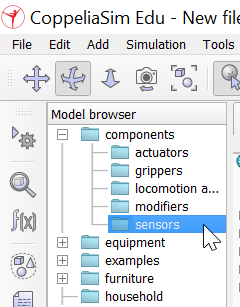
\includegraphics{figures/selecting_sensor_componant.png}}
        \quad
        \subfloat[selction accelerometer and a gyroscope sensor.]{%
            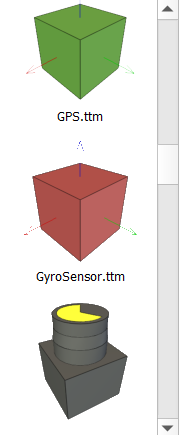
\includegraphics{figures/selecting_gyro_acc_componant.png}}
        \caption{Creating IMU.}
        \label{fig:creating_IMU}
    \end{figure}

To combine the accelerometer and a gyroscope sensor and make a single IMU we need to change the LUA script attached with every sensor. Although it was possible just to drag and drop the sensors but we wanted to create a custom script to add a single unit IMU to incorporate our custom simulation control panel. we will discuss the control panel later on in the upcoming section. 

\subsubsection{Making IMU}

We created a custom IMU combining gyroscope and accelerometer in a separate scene. To do that we selected the gyrosensor script as our base script. Then we added the accelerometer into the scene with the gyrosensor. Both of the components Lua scripts were auto-generated which can sense and collect data by the software. We changed the Lua script for both of the gyrosensor and accelerometer to get the sensor data out of the software and saved in a .txt file. When we are satisfied with our work, we saved the whole script as a new sensor names IMU. This IMU now consists of one accelerometer and one gyroscope also we can add 1  to 16 number of IMU from our custom control panel.

\begin{figure}[h]
  \centering
    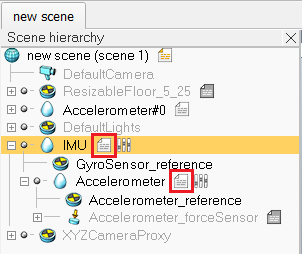
\includegraphics[width=8cm]{figures/IMU_Creation.png}
    \caption{IMU Creation.}
\end{figure}

It is important to mention, the autogenerated script was in the non-threaded mode, if we write in nonthreaded mode all the data gets overwritten by the last sensor data. we hade to wrote threaded scripts get out of this situation.

\subsubsection{IMU pattern in a 2D plane}

In sensor fusion, the number of IMU and the position of IMU plays a very important role. For that, it was very important for was to experiment with what number of IMU in which position gives us the best result. One of our primary objectives was to try the combination of IMU (2 to 16) in the simulation. 
It was very important to try different experiments with this number of IMUs for this particular issue scope. 
[..] have explored different avenues regarding 8 real IMUs joined on a circuit board to gather real-world information, yet not utilizing various examples with various numbers of IMUs. It is a direct result of the very complex nature of the task to connect and segregate IMUs after each and every run. At that point comes the issue of calibration; which is meticulous in light of the fact that each time another IMU is joined or an IMU gets disengaged all the rest of the IMUs should be adjusted one by one.

Using a simulation instead of a real-world sensor comes handy in this type of situation. Just using a mouse click we can change the number of IMU from our custom control panel without needing any calibration or registration. To identify the patterns of IMU we need a bit of trial and testing since we didn't have any benchmark for IMU designs. We took []'s work with 8 IMUs as our base and characterized the examples for the IMUs around it. Moreover, we thought about the alignment and situating for various IMUs for a genuine gadget, which in the long run helped us to settle the examples. 

The accompanying figures give a diagram of the pattern designs for the IMUs:

\begin{figure}[h!]
  \centering
  \begin{subfigure}[b]{0.2\linewidth}
    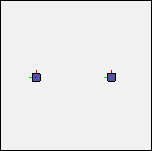
\includegraphics[width=\linewidth]{figures/IMU2.png}
    \caption{2 IMU pattern }
  \end{subfigure}
\begin{subfigure}[b]{0.2\linewidth}
    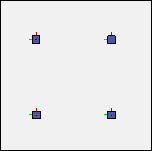
\includegraphics[width=\linewidth]{figures/IMU4.png}
    \caption{4 IMU pattern.}
  \end{subfigure}
\begin{subfigure}[b]{0.2\linewidth}
    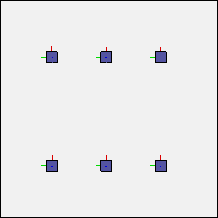
\includegraphics[width=\linewidth]{figures/IMU6.png}
    \caption{6 IMU pattern.}
  \end{subfigure}
\begin{subfigure}[b]{0.2\linewidth}
    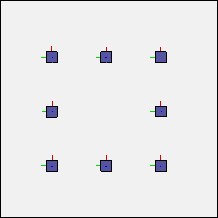
\includegraphics[width=\linewidth]{figures/IMU8.png}
    \caption{8 IMU pattern.}
  \end{subfigure}

 \begin{subfigure}[b]{0.2\linewidth}
    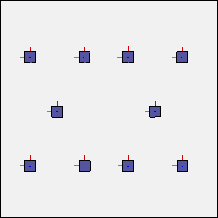
\includegraphics[width=\linewidth]{figures/IMU10.png}
    \caption{10 IMU pattern.}
  \end{subfigure}
  \begin{subfigure}[b]{0.2\linewidth}
    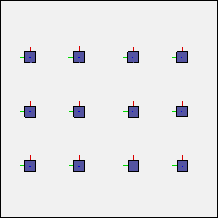
\includegraphics[width=\linewidth]{figures/IMU12.png}
    \caption{12 IMU pattern.}
  \end{subfigure}
  \begin{subfigure}[b]{0.2\linewidth}
    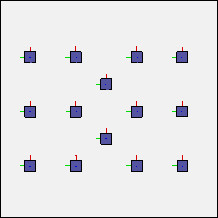
\includegraphics[width=\linewidth]{figures/IMU14.png}
    \caption{14 IMU pattern.}
  \end{subfigure}
  \begin{subfigure}[b]{0.2\linewidth}
    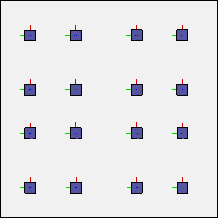
\includegraphics[width=\linewidth]{figures/IMU16.png}
    \caption{16 IMU pattern}
  \end{subfigure}

  \caption{Number of IMU position on a 2D plane.}
  \label{fig:IMU_pattern}
\end{figure}



Although we initially try to test every pattern from 1 to 16 but we end up using an even number of IMUs for our purpose to reduce the time for CNN testing and there was no significant difference from changing 2 IMU to 3 IMU then 4 IMU. 


\subsection{Simulation Path}

As we are prediction position and orientation of an object, we need a path in our simulation where our dummy object will go through. Therefore creating a simulated path as close as possible to real trajectory was one of the main concerns. Our path has to be in such a way where our object can move with 6Dof. In our simulation tool the path controllers the position and orientation of the moving object in our case the 2D plane. We need to create the paths with multiple rotation and elevation where our object will move and we can collect the data of the position and orientation, in short, the pose of the object.

\begin{figure}[h]
  \centering
    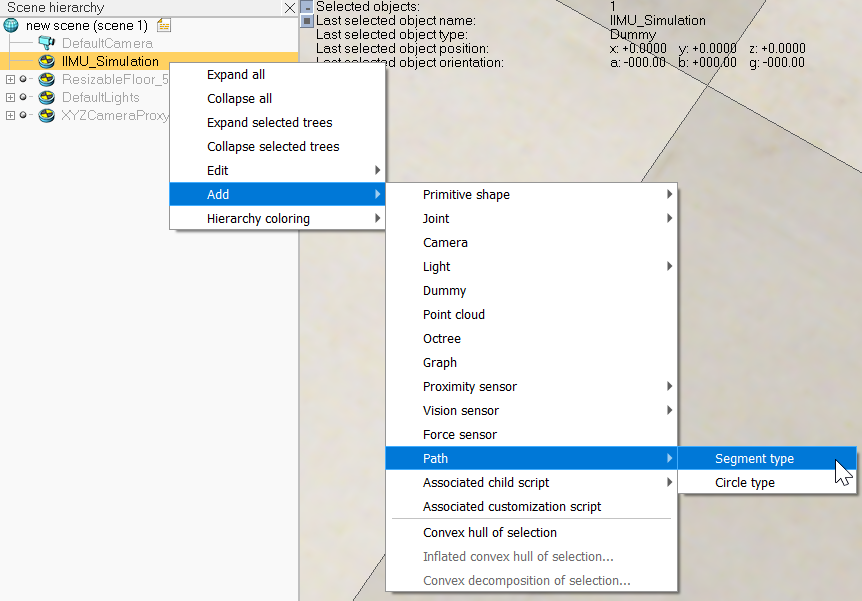
\includegraphics[width=\linewidth]{figures/pathCreation.png}
    \caption{Path Creation.}
\label{fig:Path_creation}
\end{figure}


We need a large amount of dataset to train our Neural Network for that our path has to be long enough with orientation, with elevation gain and loss to generate the data. Meaning our plane with the IMU and dummy object will go up and down, left and right rotation along the path. These features need to ensure by the path design itself. The path design also facilitates other features slike roll, pitch, and yaw. 

\subsubsection{Dummy Object}
To control our simulation environment we need a control panel, to do that we need an entry point. The creation of a dummy object makes the process easier. we need to add our customize script to the dummy object script to make our control panel. that's why adding a dummy object is very important. The detail about the control panel will be discussed in the upcoming section.
We can simply add a dummy object from the simulation tool using the following steps: 

\begin{enumerate}
  \item  Navigate to the ‘Scene hierarchy’ pane.
  \item  Right click on the scene name.
  \item Go to ‘Add’ and click on ‘Dummy’
\end{enumerate}



\begin{figure}[h!]
  \centering
  \begin{subfigure}[b]{0.4\linewidth}
    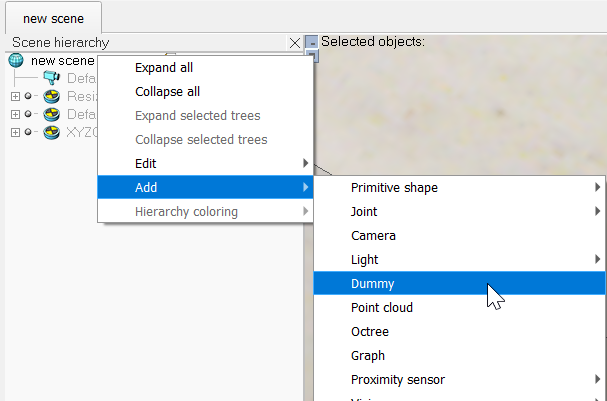
\includegraphics[width=\linewidth]{figures/addingDummyObject.png}
    \caption{Adding Dummy Object }
  \end{subfigure}
\quad
\begin{subfigure}[b]{0.4\linewidth}
    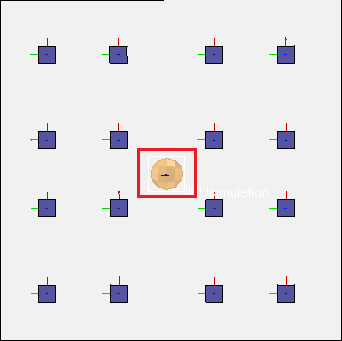
\includegraphics[width=\linewidth]{figures/DummyObjectinaPlane.png}
    \caption{Dummy Object in a Plane.}
  \end{subfigure}
 \caption{Dummy Object.}
  \label{fig:Dummy_object}
\end{figure}

After creating the dummy object we named it IMU Simulation  and we placed it in the center  (x, y, z : 0, 0, 0)  of the plane.


\subsubsection{Creating the path for the plane}

The path creation process was really time-consuming. In the beginning, we started just adding a default path from the simulation tool. There are 2 types of paths in the tool one is circular path another is the segmented path. As we needed path with many orientation and elevation we selected the segmented path showed in figure ~\ref{fig:Path_creation}.
The following steps are taken to add a segmented path in the scene:

\begin{enumerate}
  \item Go to the ‘Scene hierarchy’ pane.
  \item Right-click on IMU Simulation.
  \item Go to ‘Add’ and then go to ‘Path’.
  \item Click on ‘Segment type’ to create the primitive path.
\end{enumerate}

The segmented path just adds a straight line in the scene. At first, we added many segmented paths in the scene but when we tried to join them together it was cumbersome.
Then we decided to modify a single segmented path by adding many path control points and give it random elevation, orientation, and trajectory. To do that we need to go to the section called Path edit mode.

\subsubsection{Path Control Points}


In order to manipulate our segmented path we took a single segmented path and created many path points. Adding path points is fairly easy on the simulation tool.
Select the path from the scene.

\begin{figure}[h!]
  \centering
  \begin{subfigure}[b]{0.5\linewidth}
    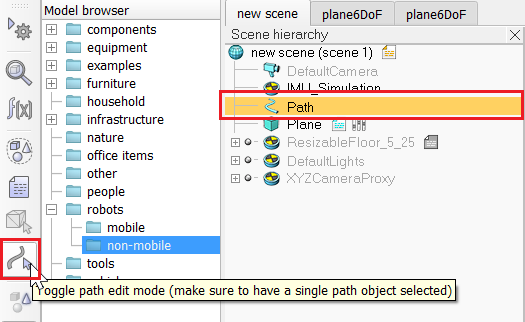
\includegraphics[width=\linewidth]{figures/PathControllPoint.png}
    \caption{Adding Path Control Points}
  \end{subfigure}
\quad
\begin{subfigure}[b]{0.5\linewidth}
    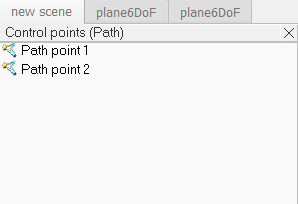
\includegraphics[width=\linewidth]{figures/PathControllPointsPane.png}
    \caption{After Path Controll Points are added.}
  \end{subfigure}
 \caption{Path Control Points.}
  \label{fig:PathControlPoint}
\end{figure}

\begin{enumerate}
  \item Click the path edit mode shown in the figure ~\ref{fig:PathControlPoint}
  \item Go to the control point section and right-click on it.
  \item From the menu, select Insert new control point after selection.
\end{enumerate}

We repeated these steps many times to make our path longer as we needed. 

The new point gets made right on the last point, or essentially put the point we chose to include the new point. To move the recently included point, from the outset we have to choose the point and afterward switch 'Object/Item shift' button on the top control panel. After we selected a control point in the scene, we just drag and drop in our desired position. This choice permits moving any article in the scene along with all the three-axis. Two kinds of movement are permitted through this process:

\begin{enumerate}
  \item Move an object along the X-axes and Y-axes by using the mouse; by simple drag and drop.
  \item Right-click on IMU Simulation.
  \item Press ‘CTL’ in the keyboard and moving the cursor up and down to move the object along Z-axis.
\end{enumerate}

We had to do these steps for every control points over our whole path.


\subsubsection{Path Orientation}

After we created the long path we run the simulation. The simulation was running well and we collected 20 minutes of simulation data. When we were analyzing the data we found that the object orientating in one axis. As we need 6Dof we can not take the data from the simulation. 
After investigating we found to change the orientation of our plane we need to change in the path control points. But, the method or the ability to add a configuration script to adjust the path Control points orientation is not available automatically from the tool. We need to change every control point we added in our simulation path. This was a time-consuming process. The longer the path the more control point we had to change. After a considerable amount of time, we change the control points and run the simulation again. This time our plane was oriented along the 3 axes but there was a problem. The object was only changing its orientation only at the control point but not along the path. For better explanation lets say, The plane was moving from control point A to control point B then to control point C. The plane is only changing its orientation axis when it reaches the control point B and keeps its orientation along the path From B to C and then change its orientation again in point C. This is not what we wanted.

We tried to solve this problem by turning on the "Automatic Orientation" checkbox in the path edit mode dialog box for orientation. By default, this box was checked. With this activated option, the object that moves along the path should frequently change its angles. But in simulation, it does not. The object only keeps the roll but not yaw and pitch. The characteristics of 6 
DoF are thus violated.






%\begin{figure}[h!]
%  \centering
%  \begin{subfigure}[b]{0.4\linewidth}
%    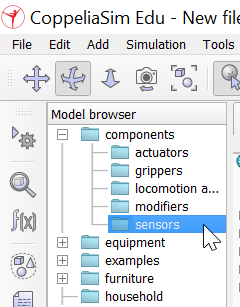
\includegraphics[width=\linewidth]{figures/selecting_sensor_componant.png}
%    \caption{Coffee.}
%  \end{subfigure}
%  \begin{subfigure}[b]{0.4\linewidth}
%    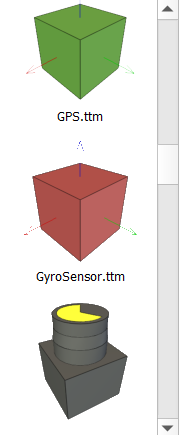
\includegraphics[width=\linewidth]{figures/selecting_gyro_acc_componant.png}
%    \caption{More coffee.}
%  \end{subfigure}
%  \caption{The same cup of coffee. Two times.}
%  \label{fig:coffee}
%\end{figure}

